\documentclass{article}

% 使用ctex宏包来支持中文
\usepackage[UTF8]{ctex}

% 设置页面尺寸和边距
\usepackage[letterpaper,top=2cm,bottom=2cm,left=3cm,right=3cm,marginparwidth=1.75cm]{geometry}

% 引用其他宏包
\usepackage{amsmath}
\usepackage{graphicx}
\usepackage[colorlinks=true, allcolors=blue]{hyperref}
\usepackage{float}
\usepackage{afterpage}
\usepackage{natbib}
\usepackage{hyperref}
\usepackage{appendix}
\usepackage{listings}

\lstset{
  backgroundcolor=\color{white},
  basicstyle=\ttfamily\footnotesize,
  breakatwhitespace=false,
  breaklines=true,
  captionpos=b,
  commentstyle=\color{mygreen},
  deletekeywords={...},
  escapeinside={\%*}{*)},
  frame=single,
  keepspaces=true,
  keywordstyle=\color{blue},
  language=Python,
  morekeywords={*,...},
  numbers=left,
  numbersep=5pt,
  numberstyle=\tiny\color{mygray},
  rulecolor=\color{black},
  showspaces=false,
  showstringspaces=false,
  showtabs=false,
  stepnumber=2,
  stringstyle=\color{mymauve},
  tabsize=2,
  title=\lstname
}


\bibliographystyle{plainnat}

\title{“机器学习公平性”文献阅读报告}
\author{温兆和 10205501432}

\begin{document}
\maketitle

在《社会计算》课程第八周的学习当中,我们接触了“机器学习的公平性”这一话题。

\section{文献阅读}
周二的实验课上,我们在树扬老师的带领下阅读了一些相关的文献。

\subsection{分类问题中的公平性}

Ninareh Mehrabi、Fred Morstatter、Nripsuta Saxena、Kristina Lerman和Aram Galstyan的\textit{A Survey on Bias and Fairness in Machine Learning}\cite{1}以一种像是文献综述的方式系统地梳理了公平的不同定义、偏见的不同种类、评价算法是否公平的方法以及近年来科学家们提出的消除机器学习中的不公平现象的方法,最后还展望了机器学习不公平领域的机遇和挑战,这极大地加深了我对“机器学习公平性”的认识。以前我只是在导论课或者专业英语课上听说过这个概念,当时我对“不公平”的理解仅仅停留在“美国的监狱在评估重刑犯是否适合出狱时倾向于把能够释放的黑人囚犯判断为不能释放”,对不公平产生的原因的认识也仅仅是“所有的不公平应该都是数据集有问题,模型、算法和训练过程本身应该是很客观的”。但是这篇文章告诉我们,不公平不仅可能来源于数据本身存在的历史和社会偏见,还有可能出自于数据测量和聚合处理方式的不恰当,甚至算法设计选择、优化函数的使用和正则化。

此外,“公平”的含义也是很丰富的。如果要求对相似的个体给出相似的预测结果,那就是“个体公平性”,如在个体属于不同人口群体时要求决策公平或是在决策过程中不显式地使用任何受保护属性。如果只是要求对不同的群体平等,那就是群体公平性,比如要求对于受保护和非受保护(如男性和女性)的群体成员正例被分配给正结果的概率应相等。而子群体公平性则要求模型在个体公平和群体公平之间达到平衡。

这篇文章还介绍了一些在机器学习中实现公平性的方法。我们可以在训练前通过转换数据来避免偏见。既然数据集的产生受到数据集策划者决策的影响,许多科学家就提出对每个数据集创建一个表格,记录数据集的创建方法、特征和动机,以便于回溯出数据集中可能出现的偏差。目前也已经有了一些探索数据集中潜在的偏见的方法。我们也能在训练时修改算法来消除歧视,比如通过改进多任务学习框架或分离分类系统实现公平分类,或是在回归分析中引入公平性惩罚。我们还能在训练后利用没有参与训练的保留集来达到公平。

文章末尾说到,机器学习公平性还面临着诸多挑战。一类是人文层面的。比如,公平有着各种不同的定义,而各种意义下的公平是很难同时达到的。此外,“公平”和“公正”也有差别。举例来说,我们用一个包含“存款多少”这一属性的数据集来训练模型,评判是否值得借贷给一个人,那么存款更多的人可能更容易得到一个creditworthy的评价。这显然是不公平的,但是一个拥有更多存款的人的确更有可能按时归还贷款,如果存款多的人和存款少的人被判为正例的概率相同,那显然是不公正的。我认为,所有的模型毕竟是为了解决实际问题而建立的,面对这一类“人文层面”的挑战,我们或许可以具体情况具体分析,根据实际需要来确定最应该采用哪一种对“公平”的定义。还有一类挑战是我们仍然没有找到从任意一个数据集中探索出不公平现象的通法,这一类问题的解决有赖于技术发展。

Muhammad Bilal Zafar、Isabel Valera、Manuel Gomez-Rodriguez和Krishna P. Gummadi的\textit{Fairness Constraints:A Flexible Approach for Fair Classification}\cite{2}还详细介绍了一种灵活的基于约束的框架,基于边界的分类器的设计,这有助于实现公平。

\subsection{排序问题和推荐系统中的公平性}
Ashudeep Singh和Thorsten Joachims的\textit{Fairness of Exposure in Rankings}\cite{3}探讨了排序中的公平性问题,而推荐系统中的公平性正是基于排序的公平性的。

Yunqi Li、Yingqiang Ge和Yongfeng Zhang的\textit{Tutorial on Fairness of Machine Learning in Recommender Systems}\cite{4}则大致介绍了推荐系统中对公平性的理解和实现公平性的方法,这更是让我打开了眼界。不同于分类问题,在排序问题中,公平的评价准则变成了不同群体在排序结果中的曝光程度是否均匀。而在推荐系统中,不仅仅是用户和物品之间的关系,还包括了其他相关方,比如平台的拥有者、广告商等。因此,推荐系统的公平性不仅仅要考虑用户和物品之间的公平性,还需要考虑到其他相关方的利益。这些目标还可能是相互冲突的,需要在它们之间进行权衡。为了实现排序问题甚或推荐系统的公平性,我们不仅可以不依赖于现有的模型或算法重新构建模型,还可以在排序后调整生成的排序结果(Re-ranking),以确保公平性或其他性能指标的提高。

\section{一个小实验}
在阅读完文献后,我也忍不住亲手探索和消除一下机器学习中的不公平。我使用了AIF360这个工具,它在参考文献\cite{1}和\cite{4}中都被提到。使用不公平问题中很经典的German Credit数据集,它包含了一千个德国人的性别、年龄、收入等信息,以及他们的信用评级(好和不好)。AIF360中有自带的工具去判断和消除机器学习中的不公平。我分别把性别(sex)和年龄(age)作为被保护属性,把“性别为男性”和“年龄大于二十五岁”设为特权条件。我使用了两个公平性指标,其中一个是不公平影响(Disparate Impact)指标,它是非特权群体与特权群体中有利结果的概率之比,越接近于一表示越公平;还有一个是Statistical Parity Difference (SPD),它衡量了不同群体之间的平均预测值之差,越接近零越公平。

\subsection{不公平现象的探索}
我们先来看看学习过程中是否产生了不公平。代码运行的结果如下图所示:
\begin{figure}[h]
    \centering
    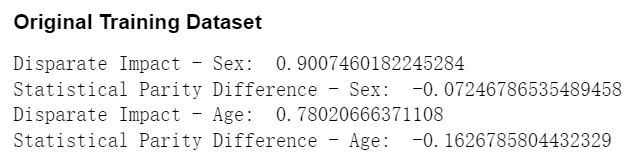
\includegraphics[width=0.49\linewidth]{img/image1.png}
    \caption{不公平探索结果}
    \label{fig:enter-label}
\end{figure}
可以看出,如果我们把“性别”作为被保护属性,那它的DI指标和SPD指标分别是$0.9$和$-0.07$,说明相对于男性来说,女性得到有利结果的概率相对少一点;然而,如果把年龄作为被保护属性,我们会看到更加严重的不公平现象:年龄较小的人得到有利结果的概率比年龄较大的要小得更多。

\subsection{不公平性的消除}

接下来我们就试着消除这些不公平。我们使用重新加权方法(Reweighting)和去偏方法(Disparate Impact Remover)来消除不公平。其中前者的思想是调整样本的权重,使得不同群体之间的分布更加平衡;而后者通过修改训练数据集中的样本,使得敏感属性对模型预测结果的影响减弱,从而减少不公平。我们分别把年龄和性别作为敏感属性运用这两种方法。除了两种方法各自的效果,我们还关心消除一个被保护属性的不公平时会对另一个属性的公平性产生什么样的影响。

我们先来看重新加权方法的实验结果:
\begin{figure}[h]
    \centering
    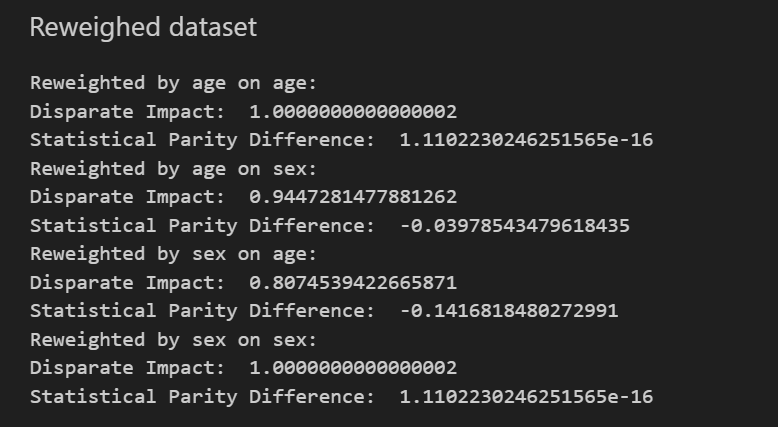
\includegraphics[width=0.58\linewidth]{img/image2.png}
    \caption{重新加权方法的实验结果}
    \label{fig:enter-label}
\end{figure}

可以看出,分别把性别和年龄两个属性作为敏感属性进行重新加权,最后相应属性上的不公平现象都几乎被彻底地消除了:DI指标无限接近于$1$,SPD指标无限接近于$0$。与此同时,如果把性别作为敏感属性,年龄属性上的DI指标从$0.78$提升到了$0.8$,SPD指标从$-0.16$被压缩到了$-0.14$。也就是说,当我们试图用重新加权方法消除性别属性上的不公平性时,年龄属性上的不公平性也在一定程度上得到了缓解。而当我们消除年龄属性上的不公平时,也能在性别属性上看到类似的现象。

接着再试试去偏方法:
\begin{figure}[h]
    \centering
    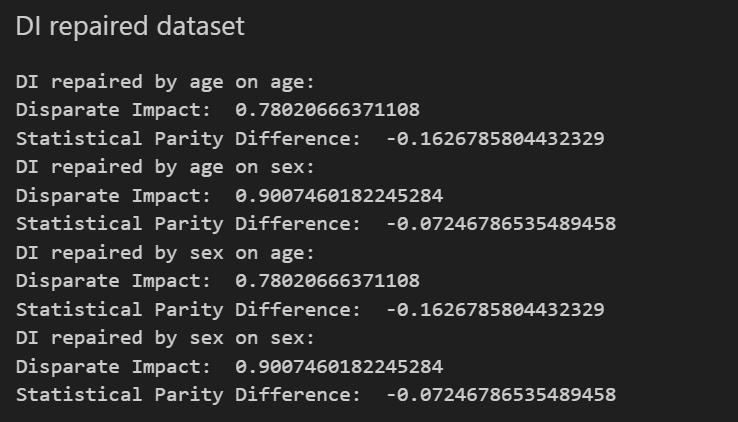
\includegraphics[width=0.58\linewidth]{img/image3.png}
    \caption{Enter Caption}
    \label{fig:enter-label}
\end{figure}

和去偏前的结果比较后可以看出,至少在这个German Credit数据集上,去偏方法没有起到什么作用。

\section*{附录}
\appendix

\section{需要安装的工具包}
实验中需要用到的主要工具有\lstinline{pandas}、\lstinline{sklearn}和\lstinline{aif360}。具体如下:
\begin{lstlisting}
import pandas as pd
from sklearn.model_selection import train_test_split
from sklearn.linear_model import LogisticRegression
from sklearn.metrics import classification_report
from aif360.datasets import GermanDataset
from aif360.metrics import BinaryLabelDatasetMetric
from aif360.explainers import MetricTextExplainer
from aif360.algorithms.preprocessing import Reweighing
from aif360.algorithms.preprocessing import DisparateImpactRemover
from IPython.display import Markdown, display
\end{lstlisting}

\section{不公平现象的探索相关代码}
\begin{lstlisting}
# 加载数据集,将性别和年龄设置为受保护属性
dataset_orig = GermanDataset(
    protected_attribute_names=['sex', 'age'],
    features_to_drop=['personal_status']        # 忽略与个人状态有关的属性
)

# 将数据集拆分为训练集和测试集
dataset_orig_train, dataset_orig_test = dataset_orig.split([0.7], shuffle=True)

# 定义特权组和非特权组
privileged_groups_sex = [{'sex': 1}]
unprivileged_groups_sex = [{'sex': 0}]
unprivileged_groups_age = [{'age': 0}]
privileged_groups_age = [{'age': 1}]

# 使用 BinaryLabelDatasetMetric 计算公平性指标
metric_orig_train_age = BinaryLabelDatasetMetric(dataset_orig_train, 
                                             unprivileged_groups=unprivileged_groups_age,
                                             privileged_groups=privileged_groups_age)
metric_orig_train_sex = BinaryLabelDatasetMetric(dataset_orig_train, 
                                             unprivileged_groups=unprivileged_groups_sex,
                                             privileged_groups=privileged_groups_sex)
display(Markdown("#### Original Training Dataset"))
print("Disparate Impact - Sex: ", metric_orig_train_sex.disparate_impact())
print("Statistical Parity Difference - Sex: ", metric_orig_train_sex.statistical_parity_difference())
print("Disparate Impact - Age: ", metric_orig_train_age.disparate_impact())
print("Statistical Parity Difference - Age: ", metric_orig_train_age.statistical_parity_difference())
\end{lstlisting}

\section{重新加权方法相关代码}
\begin{lstlisting}
RW_age = Reweighing(unprivileged_groups=unprivileged_groups_age,
                privileged_groups=privileged_groups_age)
dataset_transf_train_age = RW_age.fit_transform(dataset_orig_train)

RW_sex = Reweighing(unprivileged_groups=unprivileged_groups_sex,
                privileged_groups=privileged_groups_sex)
dataset_transf_train_sex = RW_sex.fit_transform(dataset_orig_train)

metric_transf_train_aa = BinaryLabelDatasetMetric(dataset_transf_train_age, 
                                               unprivileged_groups=unprivileged_groups_age,
                                               privileged_groups=privileged_groups_age)
metric_transf_train_as = BinaryLabelDatasetMetric(dataset_transf_train_age, 
                                               unprivileged_groups=unprivileged_groups_sex,
                                               privileged_groups=privileged_groups_sex)

metric_transf_train_sa = BinaryLabelDatasetMetric(dataset_transf_train_sex, 
                                               unprivileged_groups=unprivileged_groups_age,
                                               privileged_groups=privileged_groups_age)

metric_transf_train_ss = BinaryLabelDatasetMetric(dataset_transf_train_sex, 
                                               unprivileged_groups=unprivileged_groups_sex,
                                               privileged_groups=privileged_groups_sex)

display(Markdown("#### Reweighed dataset"))
print("Reweighted by age on age:")
print("Disparate Impact: ", metric_transf_train_aa.disparate_impact())
print("Statistical Parity Difference: ", metric_transf_train_aa.statistical_parity_difference())
print("Reweighted by age on sex:")
print("Disparate Impact: ", metric_transf_train_as.disparate_impact())
print("Statistical Parity Difference: ", metric_transf_train_as.statistical_parity_difference())
print("Reweighted by sex on age:")
print("Disparate Impact: ", metric_transf_train_sa.disparate_impact())
print("Statistical Parity Difference: ", metric_transf_train_sa.statistical_parity_difference())
print("Reweighted by sex on sex:")
print("Disparate Impact: ", metric_transf_train_ss.disparate_impact())
print("Statistical Parity Difference: ", metric_transf_train_ss.statistical_parity_difference())
\end{lstlisting}

\section{去偏方法相关代码}
\begin{lstlisting}
di_repairer_sex = DisparateImpactRemover(repair_level=1.0, sensitive_attribute='sex')
di_repairer_age = DisparateImpactRemover(repair_level=1.0, sensitive_attribute='age')

dataset_transf_train_di_sex = di_repairer_sex.fit_transform(dataset_orig_train)
dataset_transf_train_di_age = di_repairer_age.fit_transform(dataset_orig_train)

metric_transf_train_di_aa = BinaryLabelDatasetMetric(dataset_transf_train_di_age, 
                                                  unprivileged_groups=unprivileged_groups_age,
                                                  privileged_groups=privileged_groups_age)
metric_transf_train_di_as = BinaryLabelDatasetMetric(dataset_transf_train_di_age, 
                                                  unprivileged_groups=unprivileged_groups_sex,
                                                  privileged_groups=privileged_groups_sex)
metric_transf_train_di_sa = BinaryLabelDatasetMetric(dataset_transf_train_di_sex, 
                                                  unprivileged_groups=unprivileged_groups_age,
                                                  privileged_groups=privileged_groups_age)
metric_transf_train_di_ss = BinaryLabelDatasetMetric(dataset_transf_train_di_age, 
                                                  unprivileged_groups=unprivileged_groups_sex,
                                                  privileged_groups=privileged_groups_sex)

display(Markdown("#### DI repaired dataset"))
print("DI repaired by age on age:")
print("Disparate Impact: ", metric_transf_train_di_aa.disparate_impact())
print("Statistical Parity Difference: ", metric_transf_train_di_aa.statistical_parity_difference())
print("DI repaired by age on sex:")
print("Disparate Impact: ", metric_transf_train_di_as.disparate_impact())
print("Statistical Parity Difference: ", metric_transf_train_di_as.statistical_parity_difference())
print("DI repaired by sex on age:")
print("Disparate Impact: ", metric_transf_train_di_sa.disparate_impact())
print("Statistical Parity Difference: ", metric_transf_train_di_sa.statistical_parity_difference())
print("DI repaired by sex on sex:")
print("Disparate Impact: ", metric_transf_train_di_ss.disparate_impact())
print("Statistical Parity Difference: ", metric_transf_train_di_ss.statistical_parity_difference())
\end{lstlisting}

\begin{thebibliography}{9}
\bibitem{1}
Ninareh Mehrabi.Fred Morstatter.Nripsuta Saxena.Kristina Lerman.Aram Galstyan.
\textit{A Survey on Bias and Fairness in Machine Learning}.
\bibitem{2}
Muhammad Bilal Zafar.Isabel Valera.Manuel Gomez-Rodriguez.Krishna P. Gummadi.
\textit{Fairness Constraints:A Flexible Approach for Fair Classification}.
\bibitem{3}
Ashudeep Singh.Thorsten Joachims.
\textit{Fairness of Exposure in Rankings}.
\bibitem{4}
Yunqi Li.Yingqiang Ge.Yongfeng Zhang.
\textit{Tutorial on Fairness of Machine Learning in Recommender Systems}.

\end{thebibliography}

\end{document}